% Created 2024-08-12 Mon 19:55
% Intended LaTeX compiler: xelatex
\documentclass[11pt]{article}
\usepackage{hyperref}
% TIPS
% \substack{a\\b} for multiple lines text





% pdfplots will load xolor automatically without option
\usepackage[dvipsnames]{xcolor}

\usepackage{forest}
% two-line text in node by [two \\ lines]
% \begin{forest} qtree, [..] \end{forest}
\forestset{
  qtree/.style={
    baseline,
    for tree={
      parent anchor=south,
      child anchor=north,
      align=center,
      inner sep=1pt,
    }}}
%\usepackage{flexisym}
% load order of mathtools and mathabx, otherwise conflict overbrace

\usepackage{mathtools}
%\usepackage{fourier}
\usepackage{pgfplots}
\usepackage{amsthm, mathabx,  amsmath, commath}
\usepackage{amsfonts}

\usepackage{empheq}
\usepackage{tikz}
\usetikzlibrary{arrows.meta}
\usepackage[most]{tcolorbox}

\newtheorem{theorem}{Theorem}[section]
\newtheorem{definition}{Definition}[section]
\newtheorem{corollary}{Corollary}[section]
\newtheorem{example}{Example}[section]
\newtheorem{lemma}{Lemma}[section]
\newtheorem{proposition}{Proposition}[section]

\newcommand{\bl}[1] {\boldsymbol{#1}}
\newcommand{\Wt}[1] {\stackrel{\sim}{\smash{#1}\rule{0pt}{1.1ex}}}
\newcommand{\wt}[1] {\widetilde{#1}}


%For boxed texts in align, use Aboxed{}
%otherwise use boxed{}

\DeclareMathSymbol{\widehatsym}{\mathord}{largesymbols}{"62}
\newcommand\lowerwidehatsym{%
  \text{\smash{\raisebox{-1.3ex}{%
    $\widehatsym$}}}}
\newcommand\fixwidehat[1]{%
  \mathchoice
    {\accentset{\displaystyle\lowerwidehatsym}{#1}}
    {\accentset{\textstyle\lowerwidehatsym}{#1}}
    {\accentset{\scriptstyle\lowerwidehatsym}{#1}}
    {\accentset{\scriptscriptstyle\lowerwidehatsym}{#1}}
}

\usepackage{graphicx}
    
% text on arrow for xRightarrow
\makeatletter
%\newcommand{\xRightarrow}[2][]{\ext@arrow 0359\Rightarrowfill@{#1}{#2}}
\makeatother


\def \bx {\boldsymbol{x}}
\def \ba {\boldsymbol{a}}
\def \bI {\boldsymbol{I}}
\def \bt {\boldsymbol{t}}
\def \bb {\boldsymbol{b}}
\def \bA {\boldsymbol{A}}
\def \bX {\boldsymbol{X}}
\def \bu {\boldsymbol{u}}
\def \bS {\boldsymbol{S}}
\def \bZ {\boldsymbol{Z}}
\def \bz {\boldsymbol{z}}
\def \by {\boldsymbol{y}}
\def \bw {\boldsymbol{w}}
\def \bT {\boldsymbol{T}}
\def \bS {\boldsymbol{S}}
\def \bm {\boldsymbol{m}}
\def \bW {\boldsymbol{W}}
\def \bY {\boldsymbol{Y}}
\def \bH {\boldsymbol{H}}
\def \blambda {\boldsymbol{\lambda}}
\def \bPhi {\boldsymbol{\Phi}}
\def \btheta {\boldsymbol{\theta}}
\def \bmu {\boldsymbol{\mu}}
\def \bphi {\boldsymbol{\phi}}
\def \bSigma {\boldsymbol{\Sigma}}
\def \lb {\left\{}
\def \rb {\right\}}
\def \caln {\mathcal{N}}
\def \dissum {\displaystyle\Sigma}
\def \dispro {\displaystyle\prod}
\def \E {\mathbb{E}}
\def \Q {\mathbb{Q}}
\def \V {\mathbb{V}}
\def \R {\mathbb{R}}
\def \calq {\mathcal{Q}}
\def \calg {\mathcal{G}}
\def \caln {\mathcal{N}}
\def \calr {\mathcal{R}}
\def \calm {\mathcal{M}}
\def \calc {\mathcal{C}}
\def \bcup {\bigcup}

\graphicspath{{../../books/}}
\makeindex
\definecolor{mintedbg}{rgb}{0.99,0.99,0.99}
\usepackage[cachedir=\detokenize{~/miscellaneous/trash}]{minted}
\setminted{breaklines,
mathescape,
bgcolor=mintedbg,
fontsize=\footnotesize,
frame=single,
linenos}

%% ox-latex features:
%   !announce-start, !guess-pollyglossia, !guess-babel, !guess-inputenc, caption,
%   image, !announce-end.

\usepackage{capt-of}

\usepackage{graphicx}

%% end ox-latex features


\author{Paul E. McKenny}
\date{\today}
\title{Is Parallel Programming Hard, And, If So, \\What Can You Do About It?}
\hypersetup{
 pdfauthor={Paul E. McKenny},
 pdftitle={Is Parallel Programming Hard, And, If So, \\What Can You Do About It?},
 pdfkeywords={},
 pdfsubject={},
 pdfcreator={Emacs 31.0.50 (Org mode 9.8-pre)}, 
 pdflang={English}}
\begin{document}

\maketitle
\tableofcontents

\section{Deferred Processing}
\label{sec:orgab30855}
\subsection{Running Example}
\label{sec:org386f3e0}
The value looked up and returned will also be a simple integer, so that the data structure is as shown
in Figure \ref{9.1}, which directs packets with address 42 to interface 1, address 56 to interface 3,
and address 17 to interface 7.

\begin{center}
\includegraphics[width=.99\textwidth]{../images/perfbook/3.png}
\captionof{figure}{\label{9.1}Pre-BSD Packet Routing List}
\end{center}

\begin{listing}[htbp]
\begin{minted}[]{c}
struct route_entry {
    struct cds_list_head re_next;
    unsigned long addr;
    unsigned long iface;
};
CDS_LIST_HEAD(route_list);

unsigned long route_lookup(unsigned long addr)
{
    struct route_entry *rep;
    unsigned long ret;

    cds_list_for_each_entry(rep, &route_list, re_next) {
        if (rep->addr == addr) {
            ret = rep->iface;
            return ret;
        }
    }
    return ULONG_MAX;
}

int route_add(unsigned long addr, unsigned long interface)
{
    struct route_entry *rep;

    rep = malloc(sizeof(*rep));
    if (!rep)
        return -ENOMEM;
    rep->addr = addr;
    rep->iface = interface;
    cds_list_add(&rep->re_next, &route_list);
    return 0;
}

int route_del(unsigned long addr)
{
    struct route_entry *rep;

    cds_list_for_each_entry(rep, &route_list, re_next) {
        if (rep->addr == addr) {
            cds_list_del(&rep->re_next);
            free(rep);
            return 0;
        }
    }
    return -ENOENT;
}
\end{minted}
\caption{\label{l9.1}Sequential Pre-BSD Routing Table}
\end{listing}

Listing \ref{l9.1} (\texttt{route\_seq.c}) shows a simple single-threaded implementation corresponding to Figure \ref{9.1}.
\subsection{Reference Counting}
\label{sec:org8630a72}
\begin{listing}[htbp]
\begin{minted}[]{c}
struct route_entry {
    atomic_t re_refcnt;
    struct route_entry *re_next;
    unsigned long addr;
    unsigned long iface;
    int re_freed;
};
struct route_entry route_list;
DEFINE_SPINLOCK(routelock);

static void re_free(struct route_entry *rep)
{
    WRITE_ONCE(rep->re_freed, 1);
    free(rep);
}

unsigned long route_lookup(unsigned long addr)
{
    int old;
    int new;
    struct route_entry *rep;
    struct route_entry **repp;
    unsigned long ret;

retry:
    repp = &route_list.re_next;
    rep = NULL;
    do {
        if (rep && atomic_dec_and_test(&rep->re_refcnt))
            re_free(rep);
        rep = READ_ONCE(*repp);
        if (rep == NULL)
            return ULONG_MAX;
        do {
            if (READ_ONCE(rep->re_freed))
                abort();
            old = atomic_read(&rep->re_refcnt);
            if (old <= 0)
                goto retry;
            new = old + 1;
        } while (atomic_cmpxchg(&rep->re_refcnt,
                                old, new) != old);
        repp = &rep->re_next;
    } while (rep->addr != addr);
    ret = rep->iface;
    if (atomic_dec_and_test(&rep->re_refcnt))
        re_free(rep);
    return ret;
}
\end{minted}
\caption{\label{l9.2}Reference-Counted Pre-BSD Routing Table Lookup (BUGGY)}
\end{listing}

Starting with Listing \ref{l9.2}, line 2 adds the actual reference counter, line 6 adds a \texttt{->re\_freed}
use-after-free check field, line 9 adds the \texttt{routelock} that will be used to synchronize concurrent
updates, and lines 11–15 add \texttt{re\_free()}, which sets \texttt{->re\_freed}, enabling \texttt{route\_lookup()} to check for
use-after-free bugs. In \texttt{route\_lookup()} itself, lines 29–30 release the reference count of the prior
element and free it if the count becomes zero, and lines 34–42 acquire a reference on the new element,
with lines 35 and 36 performing the use-after-free check.

\begin{listing}[htbp]
\begin{minted}[]{c}
int route_add(unsigned long addr, unsigned long interface)
{
    struct route_entry *rep;

    rep = malloc(sizeof(*rep));
    if (!rep)
        return -ENOMEM;
    atomic_set(&rep->re_refcnt, 1);
    rep->addr = addr;
    rep->iface = interface;
    spin_lock(&routelock);
    rep->re_next = route_list.re_next;
    rep->re_freed = 0;
    route_list.re_next = rep;
    spin_unlock(&routelock);
    return 0;
}

int route_del(unsigned long addr)
{
    struct route_entry *rep;
    struct route_entry **repp;

    spin_lock(&routelock);
    repp = &route_list.re_next;
    for (;;) {
        rep = *repp;
        if (rep == NULL)
            break;
        if (rep->addr == addr) {
            *repp = rep->re_next;
            spin_unlock(&routelock);
            if (atomic_dec_and_test(&rep->re_refcnt))
                re_free(rep);
            return 0;
        }
        repp = &rep->re_next;
    }
    spin_unlock(&routelock);
    return -ENOENT;

}
\end{minted}
\caption{\label{l9.3}Reference-Counted Pre-BSD Routing Table Add/Delete (BUGGY)}
\end{listing}
\section{Appendices\hfill{}\textsc{ignore}}
\label{sec:org280143d}
\appendix
\subsection{Why Memory Barriers}
\label{sec:org5ac07b7}
\subsubsection{Cache Structure}
\label{sec:org4d6f602}
\begin{center}
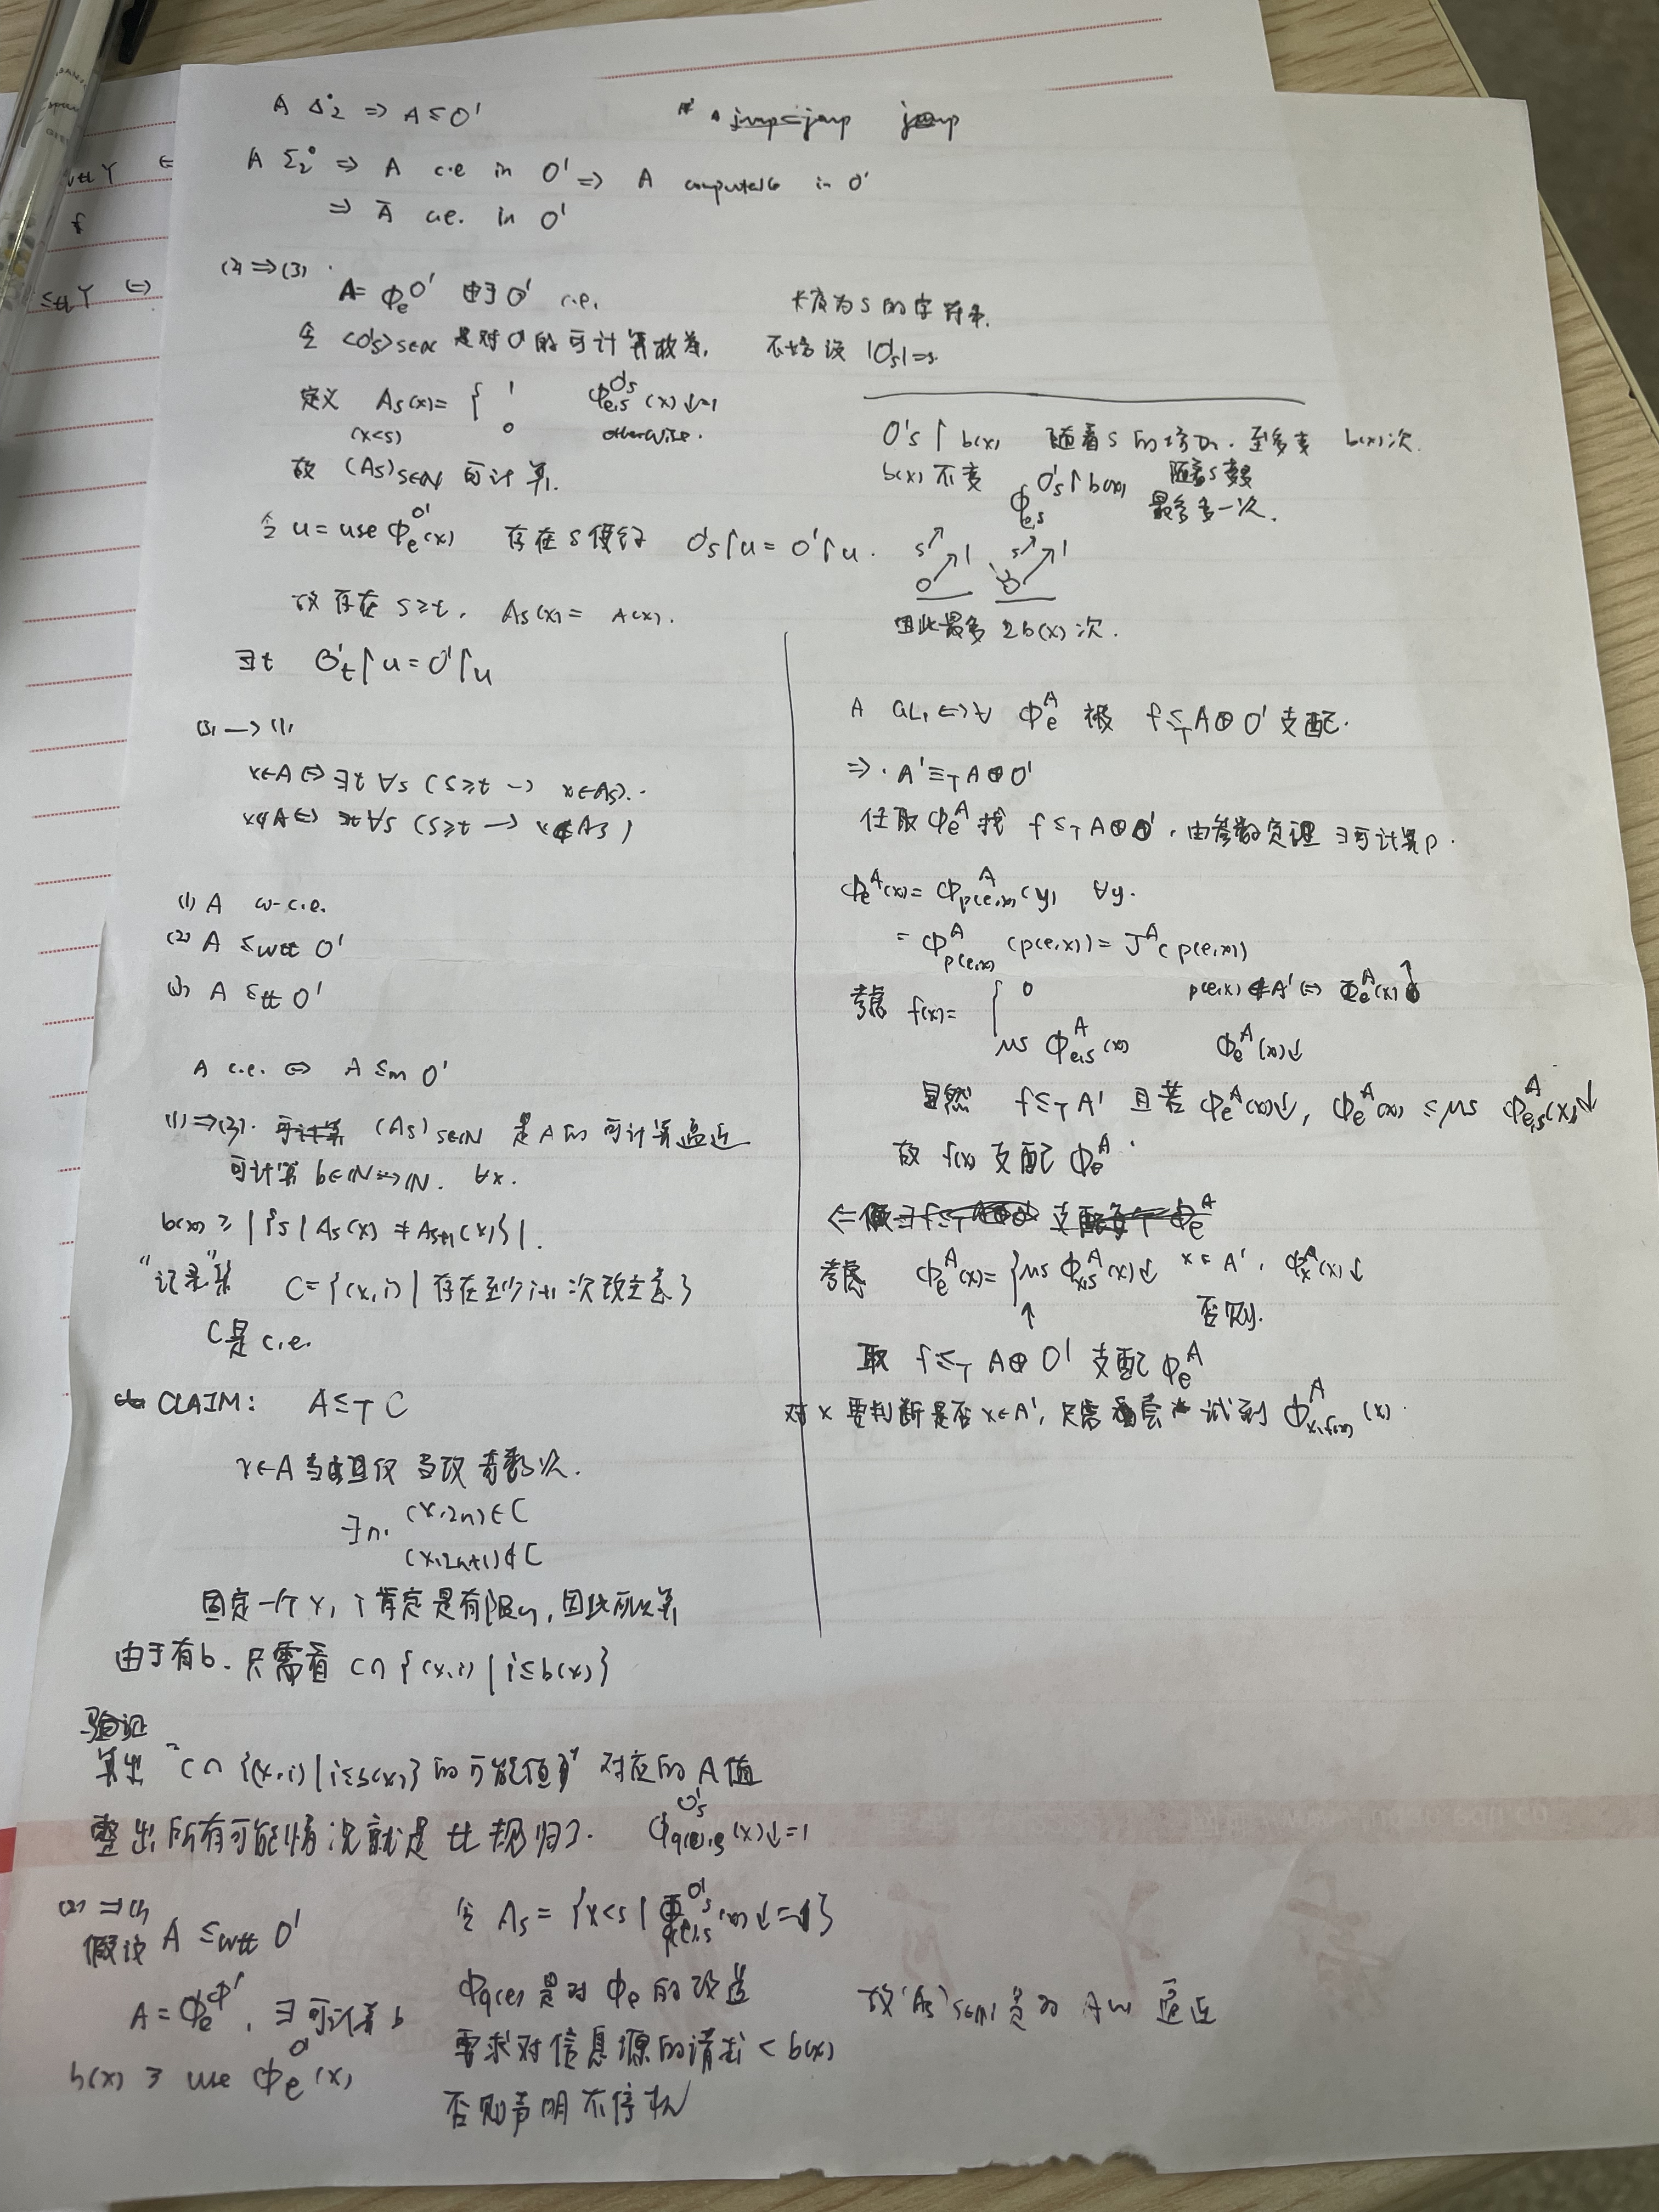
\includegraphics[width=.7\textwidth]{../images/perfbook/1.png}
\captionof{figure}{\label{}Modern Computer System Cache Structure}
\end{center}

Data flows among the CPUs’ caches and memory in fixed-length blocks called “cache lines”, which
are normally a power of two in size, ranging from 16 to 256 bytes. When a given data item is
first accessed by a given CPU, it will be absent from that CPU’s cache, meaning that a “cache
miss” (or, more specifically, a “startup” or “warmup” cache miss) has occurred. The cache miss
means that the CPU will have to wait (or be “stalled”) for hundreds of cycles while the item is
fetched from memory. However, the item will be loaded into that CPU’s cache, so that subsequent
accesses will find it in the cache and therefore run at full speed.

\begin{center}
\includegraphics[width=.8\textwidth]{../images/perfbook/2.png}
\captionof{figure}{\label{}CPU Cache Structure}
\end{center}

This cache has sixteen “sets” and two “ways” for a total of 32 “lines”, each entry containing a
single 256-byte “cache line”, which is a 256-byte-aligned block of memory.

Each box corresponds to a cache entry, which can contain a 256-byte cache line. Since the cache
lines must be 256-byte aligned, the low eight bits of each address are zero, and the choice of
hardware hash function means that the next-higher four bits match the hash line number.

What happens when it does a write? Because it is important that all CPUs agree on the value of a
given data item, before a given CPU writes to that data item, it must first cause it to be
removed, or “invalidated”, from other CPUs’ caches. Once this invalidation has completed, the
CPU may safely modify the data item. If the data item was present in this CPU’s cache, but was
read-only, this process is termed a “write miss”. Once a given CPU has completed invalidating a
given data item from other CPUs’ caches, that CPU may repeatedly write (and read) that data
item.

Later, if one of the other CPUs attempts to access the data item, it will incur a cache miss,
this time because the first CPU invalidated the item in order to write to it. This type of cache
miss is termed a “communication miss”, since it is usually due to several CPUs using the data
items to communicate (for example, a lock is a data item that is used to communicate among CPUs
using a mutual-exclusion algorithm).

Clearly, much care must be taken to ensure that all CPUs maintain a coherent view of the data.
With all this fetching, invalidating, and writing, it is easy to imagine data being lost or
(perhaps worse) different CPUs having conflicting values for the same data item in their
respective caches.
\subsubsection{Cache-Coherence Protocols}
\label{sec:orgdaaf6d5}
\begin{enumerate}
\item MESI States
\label{sec:org11fe8e5}
MESI stands for ``modified'', ``exclusive'', ``shared'', and ``invalid'', the four states a given cache
line can take on using this protocol.
\end{enumerate}
\end{document}
